\documentclass[a4paper]{article}

\usepackage[swedish]{babel}
\usepackage[T1]{fontenc}
\usepackage[utf8]{inputenc}
\usepackage{graphicx}
\usepackage{float}
\usepackage{comment}
\usepackage{appendix}
\usepackage[backend=biber, style=ieee, sorting=none]{biblatex}
%\DeclareFieldFormat{url}{\bibstring{urlfrom}\addcolon\space\url{#1}}
%\addbibresource{referenser.bib}

\newcommand\namn{Larmsystem}
\newcommand{\todo}[1]{\marginpar{TODO: #1}\vspace{1cm}}
%\newcommand{\comment}[1]{\marginpar{Comment: #1}}

\newcommand{\subsubsubsection}[1]{\paragraph{#1}\mbox{}\\}
\setcounter{secnumdepth}{4}
\setcounter{tocdepth}{4}

% Nr, författare, titel, år, url, hämtad
\newcommand{\citewebpage}[6]{\noindent [#1] #2, "#3," #4. [Online]. Tillgänglig: \url{#5},  hämtad #6}

\restylefloat{table}

\begin{document}


\thispagestyle{empty}

\begin{center}
    \parskip=14pt
    \vspace*{3\parskip}

    {\LARGE Modulärt larmsystemet}

    {\large Datateknik - Datatekniskt projekt, grupp 11

    Titus Blosse, Viktor Frideen, Nazif Kadiroglu, Markus Moen, Lukas Schiavone, Fredrik Österström

    \today}

    \rule{7cm}{0.4pt}\\
\end{center}
\newpage

\thispagestyle{empty}

\tableofcontents
\newpage

\thispagestyle{empty}

\section*{Ordlista}

\begin{description}
    \item[CAN:] Controller Area Network
    \item[IDE:] Integrated Development Environment
    \item[MD407:] Mikrodator av typen MD407
    \item[USART:] Universal Synchronous and Asynchronous Receiver-Transmitter
    \item[DICP:] Dynamic Identification Configuration Protocol
\end{description}
\newpage

\pagenumbering{arabic}

\section{Inledning}
Inbrott är ett vanligt problem i Sverige.
År 2019 anmäldes 75.250 inbrottstölder.
En minskning med 14 \% från året innan [1].
Vanliga sätt att förhindra inbrott är grannsamverkan, certifierade lås mot inbrott och hemlarm.
Larmsystem minskar risken för ett inbrott och möjliggör ytterligare minskning både i Sverige och i resten av världen.

\subsection{Syfte}
Ett modulärt larmsystem som informerar dess användare om oönskade intrång ska utvecklas.
Systemet ska lämpa sig för säkring av mindre byggnader som kontor och lägenheter.
Möjlighet ska finnas för systemets användare att anpassa systemet efter sina förutsättningar.

\subsection{Mål}

Produkten ska erbjuda ett flertal larmkomponenter som kan anslutas till en larmcentral.
Varje enhet ska kunna konfigureras och anpassas för att passa kundens specifika situation.
Till exempel ska kunden kunna justerbara antal anslutna larmkomponenter eller på vilka villkor komponenterna alarmerar.
Dessutom ska systemet vara dokumenterat och fackmannamässigt utfört med förutsättningar för expansion.

Grunden i systemet kommer vara en centralenhet till vilken användaren kan ansluta periferienheter.
Huvudsakligen kommer två periferienheter att utvecklas, ett dörrlarm och ett rörelselarm.

Dörrlarmet ska trigga ett larm då en dörr står öppen längre än ett givet tidsinterval.
Inledningsvis ska larmet sättas igång lokalt på periferienheten.
Om larmet inte hanteras inom ett givet tidsintervall vidarebefordras larmet till centralenheten.
Då kommer användaren, med hjälp av ljud och display, få ett meddelande om att larmet har löst ut.
När larmet har startat ska det krävas manuell inmatning av fyrsiffrig kod på en ansluten knapsats för att larma av.
Denna kod kommer förinstallerad på systemet men den kan ändras av användaren.

I mån av tid kommer extra funktionalitet implementeras.
Denna extra funktionalitet kommer innebära ett självlärande system, ett testläge för periferienheterna, ett lokalt larm för rörelsesensorn och ett inbyggt skydd mot återuppspelningsattacker, en attack där förövaren återger tidigare skickad data i dataintrångsyfte.


\subsection{Arbetsmetod}

Det första steget i projektarbetet var att ta fram en plan över det system som skulle konstrueras.
En skiss över de beståndsdelar systemet skulle komma att innefatta samt hur dessa skulle hänga samman togs fram.

I nästa steg delades arbetsgruppen upp i tre undergrupper som ansvarade över olika delar av projektet.
Grupperna utvecklade mjukvaran som var grunden för deras specifika område för att sedan stegvis utöka funktionaliteten.
Under utvecklingens gång ökade sammarbetet mellan grupperna då de separata mjukvarorna integrerades och gemensamt arbete blev fördelaktigt.

Mjukvaran för projektet är skriven i programmeringsspråket C, ett språk som lämpar sig väl för utveckling mot mikrodatorn MD407 vilket är den hårdvara som driver systemet.

Versionshantering har gjorts med hjälp av git.
Ett gemensamt fjärrarkiv skapades på GitHub där all kod för projektet samlades.

Majoriteten av testen utfördes direkt på hårdvaran i Chalmers lokaler.
Vissa tester har genomförts med hjälp av mjukvaran Simserver som tillåter simulering av MD407-kortet.
Funktionaliteten hos Simserver är begränsad och därför har den största delen av testerna behövts utföras i Chalmers laborationssalar.

De restriktioner som har legat på sociala sammankomster under utvecklingstiden har påverkat arbetet. Vid ett fåtal tillfällen har hela arbetsgruppen varit samlad i samma rum.
Stor del av all kommunikation kring projektet har skett via kommunikationsverktygen Zoom, Discord och Messenger.

\newpage

\section{Teknisk beskrivning}
I detta avsnitt ges en fördjupad inblick i hur systemet hänger ihop och fungerar.
Den mjuk- och hårdvara som projektet baseras på beskrivs även i mer detalj.

\subsection{Teknisk bakgrund}
Hårdvaran som systemet körs på är en MD407-mikrodator.
Mjukvaran är skriven i programmeringsspråket C.
MD407 har begränsat med minne vilket gör att programmen som skrivs för mikrodatorn bör vara små och effektiva.
C är ett lågnivå-programmeringsspråk vilket medför att programmeraren har stor kontroll över minneshanteringen i programmet.
C lämpar sig alltså för utveckling mot MD407.

Systemet kretsar kring att flera MD407 sammankopplas, en av dessa mikrodatorer agerar som centralenhet och att resterande används för att ansluta periferienheter.
MD407-korten kommunicerar via ett protokoll som baserats på CAN (Controllerar Area Network), ett protokoll för kommunikation mellan datorer.
% Ett kommunikationsprotokoll har sedan byggts ovanpå CAN som är anpassat för systemet.

\subsection{Systemöversikt}

Ett MD407-kort väljs som centralenhet för systemet.
Från denna enhet körs huvudprogrammet.
Centralenheten sköter huvudparten av systemets funktion.
Centralenheten registrerar vilka periferienheter som är anslutna, kontrollerar kontinuerligt så att inget alarm gått hos periferienheterna och läser inmatning från en ansluten dator för att styra systemet.

Två typer av periferienhet finns tillgängliga att ansluta till systemet.
Ett dörrlarm, kontrollerar huruvida en dörr är öppen eller stängd och en rörelsesensor mäter avståndet till föremålet framför den och registrerar om detta förändras.
Om dörren är öppen längre än en bestämd tid eller om rörelsesensorn registrerar en avvikelse i avstånd kommer periferienheterna larma.
Om larmet fortsätter tillräcklig länge kommer periferienheten i fråga skicka ett meddelande till centralenheten.

\begin{figure}[H]
    \centering
    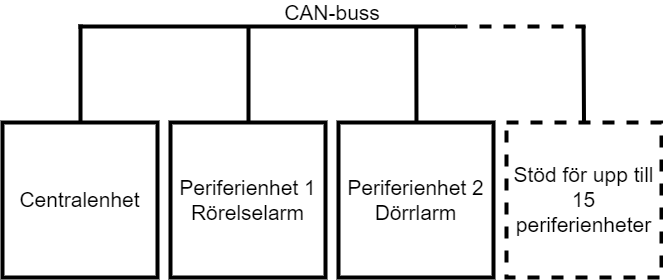
\includegraphics[width=\textwidth]{canbuss-pp.png}
    \caption{Översikt över systemet}
\end{figure}

\begin{table}[H]
    \centering
    \caption{CAN-meddelandets uppbyggnad samt ett exempel på hur ett alarm-meddelande från en periferienhet ser ut.}
    \label{tab:meddelandestruktur}

    \resizebox{\textwidth}{!}{\begin{tabular}{|c|c|c|c|c|c|c|c|c|c|c|c|c|c|c|}\hline
        \multicolumn{1}{|c|}{Riktning} & \multicolumn{6}{|c|}{Meddelande-ID} & \multicolumn{4}{|c|}{Enhets-ID} & \multicolumn{3}{|c|}{Längd} & \multicolumn{1}{|c|}{Data (8 bytes)} \\\hline
        0 & 0 & 0 & 0 & 0 & 0 & 0 & 0 & 0 & 0 & 1 & 0 & 0 & 0 & 0 \\\hline
        \multicolumn{1}{|c|}{TO\_CENTRAL} & \multicolumn{6}{|c|}{ALARM} & \multicolumn{4}{|c|}{NodeId} & \multicolumn{3}{|c|}{0} & \multicolumn{1}{|c|}{0} \\\hline
    \end{tabular}}
\end{table}

\subsubsection{Controller area network}
Ett protokoll har utvecklats för kommunikation mellan enheterna.
Basen till protokollet är CAN-meddelanden(Controller Area Network) som skickas mellan enheterna.

CAN är ett protokoll för kommunikation och hantering av meddelanden mellan enheter.
CAN-protokollet måste därför finnas hos både periferienhet och centralenhet.
Koden är därför strukturerad så att samma kod kan köras på valfri enhet oavsett typ.
Med hjälp av riktning och enhets-ID (enhets-identifikation) kan alla enheter ta emot och skicka meddelanden till godtycklig mottagare.
Varje CAN-meddelande byggs upp av fem fält:

\begin{description}
    \item[Riktning:] Detta fält anger om meddelandet går till eller från centralenheten.
    Fältet sätts till TO\_PERIPHERAL, motsvarande noll om meddelandet går från centralenhet till periferienhet och TO\_CENTRAL, motsvarande ett om meddelandet går från periferienhet till centralenhet.
    Detta fält tillåter en minskning av antalet meddelandetyper då en generell meddelandetyp som ALARM kan användas åt båda hållen.

    \item[Meddelande-ID:] Meddelanden delas upp i meddelandetyper, till exempel: ALARM och ERROR.
    Alla meddelandetyper finns samlade i en uppräkningstyp.
    Ordningen i uppräkningstypen bestämmer meddelandets prioritet.
    Ju närmare noll, desto högre prioritet.
    Samtliga meddelandetyper finns samlade i Tabell \ref{tab:meddelandetyper}.

    \item[Enhets-ID:] Varje ansluten enhet tilldelas ett unikt enhets-ID, mellan 0 och 14.
    15 är reserverat för ID-tilldelning. Ett lägre enhets-ID innebär högre prioritet.
    Centralenheten tilldelar enheterna ett ID i ordningen de anslöt sig i.

    \item[Längd:] Längd är en indikation på hur mycket data som skickas med i meddelandets datafält.
    Många meddelanden skickas med längd noll då mycket information om meddelandet kan utläsas från meddelande-ID och enhets-ID.

    \item[Data:] I detta fält lagras den data som skickas med i meddelandet.
    Ett meddelande kan lagra upp till 64 bitar av data.
\end{description}

\begin{table}[H]
    \centering
    \caption{Samtliga meddelandetyper och deras prioritet.}
    \label{tab:meddelandetyper}
    \begin{tabular}{|c|c|}\hline
      Prioritet & Meddelande-ID \\\hline
      0 & ALARM \\\hline
      1 & ERROR \\\hline
      2 & ALARM\_OFF \\\hline
      3 & POLL\_REQUEST \\\hline
      4 & POLL\_RESPONSE \\\hline
      5 & DICP\_REQUEST \\\hline
      6 & DICP\_RESPONSE \\\hline
      7 & TOL\_SET \\\hline
      8 & ACTIVE\_ON \\\hline
      9 & ACTIVE\_OFF \\\hline
    \end{tabular}
  \end{table}

Då ett meddelande ska skickas anropas en avsändarfunktion hos den enhet som vill skicka.
För varje meddelandetyp finns en unik avsändarfunktion som skapar ett CAN-meddelande med de nödvändiga parametrarna.
Funktionen lägger sedan ut meddelandet på bussen så att mottagaren kan plocka upp det.

För centralenhet och periferienhet finns unika mottagningsfunktioner.
Mottagningsfunktionen undersöker riktnings- och enhets-ID-fälten hos mottaget CAN-meddelande.
Funktionen avgör sedan hurvida mottaget meddelande berör enheten.
Om så är fallet kontrolleras meddelandetypen och en funktion för att hantera meddelandet kallas.
För varje meddelandetyp finns en unik hanteringsfunktion som utför de instruktioner meddelandet medförde.

\subsubsection{Centralenhet}
Centralenheten sköter huvuddelen av systemets funktionalitet.
Främst ansvarar den för övervaka alla anslutna enheter och alarmera om ett alarm uppstår hos någon av dem.
Om alarm uppstår kan det avvaktiveras genom att mata in en fyrsiffrig kod på ansluten knappsats.

Centralenheten både lyssnar efter meddelanden och skickar meddelanden till periferienheterna kontinuerligt.
Ett meddelande till centralenheten kan till exempel innefatta ett alarm, ny ID-förfrågan eller att det uppstått ett fel.

Centralenheten skickar kontinuerligt förfrågningar, även kallat pollingmeddelande, till periferienheterna.
Detta för att undersöka så att inga enheter kopplas bort samt för att förebygga återupspelningsattacker.
I varje pollingmeddelande skickas en tidsstämpel från centralenhetens drifttid.
Enheten som mottager pollingmeddelandet förväntas svara centralenheten inom ett visst tidsintervall.
I pollingsvaret ska tidsstämpeln återfinnas fast inverterad.
När centralenheten mottager ett pollingsvar inom tidsramen med en korrekt inverterad tidstämpel skickas ett nytt pollingmeddelande till nästa anslutna enhet.
Om korrekt pollingsvar ej mottages startas ett alarm från centralenheten.

De instruktioner som matas in av användare via ansluten konsol hanteras av centralenheten.
För att inte störa programflödet kontrolleras inmatningen av tecken periodiskt istället för att systemet väntar på inmatning från användare.
Inmatade tecken sparas i en buffer.
Då buffern är full eller en blankrad matas in av användare tolkas tecknen i buffern.
Om ett korrekt kommando har matats in kallas en funktion som hanterar kommandot.

\begin{figure}[H]
    \centering
    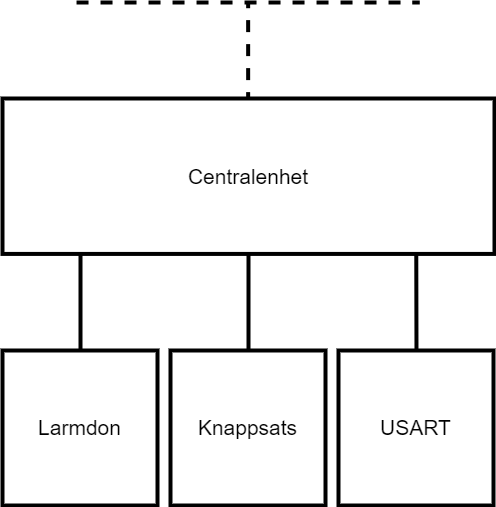
\includegraphics[width=0.5\textwidth]{central-oversikt-pp.png}
    \caption{Översikt över centralenheten och dess komponenter}
\end{figure}

%skickas för att säkerställa att enheten i fråga fortfarande är ansluten och inte larmar. I pollingmeddelandet

\subsubsection{Periferienhet}
När periferienheten initialiseras hämtas en identifierare från centralenheten via CAN.
Detta görs genom att anta en standard-identifierare 15 och att skicka ett DICP(Dynamic Identification Configuration protocol)-meddelande.
Centralenheten tilldelar periferienheten och besvarar DICP-meddelandet med den tilldelade identifikationen.
Vid framtida kommunikation använder periferienheten sig av sin unika identifierare för att skicka meddelanden.

För att inte centralenheten ska initiera ett alarm måste periferienheterna kunna svara på dess förfrågan.
Vid en förfrågan skickar centralenheten ett meddelande till en uppkopplad periferienhet.
I meddelandet anger centralenheten den lokala tiden då förfrågningen skickades.
Periferienhetens uppgift är att bitvis invertera tiden innan den besvarar meddelandet.
Centralenheten verifierar att den inverterade tiden stämmer överrens med tiden då den skickade meddelandet.
Om en avvikelse i tiden uppstår så larmar centralenheten med ett alarm.

Periferienheterna avlyssnar sina sensorer och rapporterar ett alarm till centralenheten om tröskeln för sensortypen är överskriden.
Det finns tre typer av sensorer, en dörr-, en avstånds- och en vibrationssensor.

\begin{description}
    \item[Dörrsensor:] Dörrsensorns uppgift är att upptäcka om en dörr är öppen eller stängd.
    Värdet på sensorerna läses av från PE0-12, portpinnar på MD407, som är konfigurerade med en Pull-Up-resistorer.
    Vid öppnad dörr bryts kretsen och det logiska värdet blir ett.
    Vid sluten krets är det logiska värdet på kretsen noll.

    \item[Avståndssensor:] Avståndssensorns uppgift är att upptäcka skillnader i avstånd.
    För att kunna läsa ett värde från sensorn måste en logisk etta skrivas till trig-pinnen i minst 10 \textmu s.
    Sensorn svarar med att skriva en logisk etta på echo-pinnen.
    Längden av denna logiska etta motsvarar det uppmätta avståndet.

    \item[Vibrationssensor:] Vibrationssensors uppgift är att upptäcka vibrationer.
    En vibrationssensor används ofta för att mäta böjningar, beröring, vibration eller stötar.
    Sensorn kan rapportera en vibration både analogt via A0-pinnen eller digitalt via D0-pinnen på sensorn.
    D0 används för att läsa det logiska värdet på sensorn.
    Noll motsvarar en vibration och ett motsvarar standardtillståndet.
\end{description}

Dörrsensors tröskel justeras genom att sätta det antal tillåtna sekunder som en dörr kan vara öppen.
När en dörr öppnas sparar periferienheten den aktuella tiden.
Överskrider tiden som dörren varit öppen den tillåtna tiden skapar periferienheten ett alarm.

Avståndssensorn samlar kontinuerligt in mätvärden för avståndet.
Genom att beräkna variansen på dessa mätvärden har avståndssensorn möjligheten att upptäcka en rörelse.
En varians större än tröskeln medför ett alarm.
En lägre tröskel används för att lokalt kunna alarmera.

Vibrationssensorns känslighet justeras direkt på sensorn.
Detta görs genom att ställa in en potentiometer med hjälp av en skruvmejsel.

\begin{figure}[H]
    \centering
    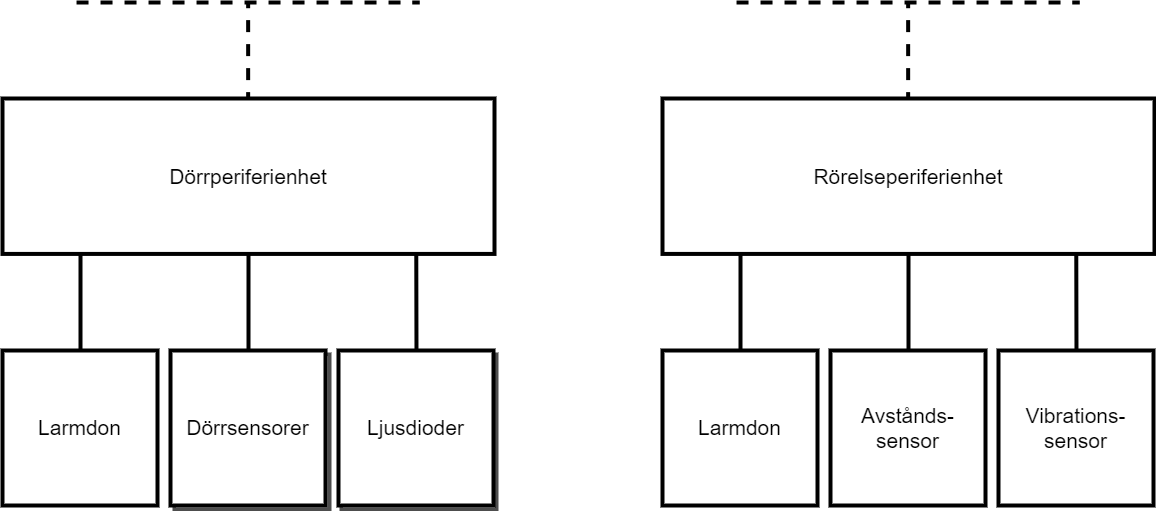
\includegraphics[width=\textwidth]{periferi-oversikt-pp.png}
    \caption{Översikt över periferienheterna och dess komponenter}
\end{figure}

\newpage

\section{Metod}
Detta kapitel beskriver hur projektet har utförts; vad som har gjorts och hur det har gjorts.
Varje delsystem gås igenom för sig men de olika komponenterna har ofta utvecklats parallellt då det finns många delar av dem som överlappar.
Att delsystemen är kompatibla och kan samarbeta med varandra är viktigt för att systemet i sin helhet ska fungera.

För att förenkla arbetet i början delades det in i tre olika delar: CAN, centralenheten och periferienheterna.
I början av projektet jobbade varje undergrupp enskilt på de olika delarna.
Senare i projektet när systemet närmade sig färdigställning återgick gruppen till att arbeta tillsammans.

\subsection{Utveckling av CAN}
Arbetet med CAN-protokollet påbörjades teoretiskt med att hitta en standard för hur meddelanden skulle vara strukturerade.
När en standard för meddelandestruktur var definierad påbörjades arbetet med att ta fram de olika meddelandetyperna.
Alla typer av meddelanden, dess funktion och dess parametrar dokumenterades och gjordes lätttillgängligt i kodbasen.
En gemensam mottagar-funktion utvecklades som kom att bli standarden för alla enheter i systemet.
Mottagaren hanterar meddelandet och tar reda på vilken typ det är genom att bryta ner meddelandet.
Beroende på meddelandetyp kallas den korresponderande funktionen.
När mottagaren var på plats påbörjades implementeringen av diverse funktionalitet.

CAN-protokollet samlar datan från en inkommande sänding i ett RX-meddelande.
Logiken och koden för att göra om ett sådant meddelande till ett CANMsg var sedan tidigare given.
Metoder för att till exempel uppdatera tolerans eller sätta antalet dörrar utvecklades.
När funktionerna var testade så lades de till i mottagarfunktionen.

För att skicka ett meddelande via CAN måste det initialiseras.
Funktioner togs fram för att på ett kompakt sätt kunna initialisera meddelanden utan behovet av att upprepa kod.
Efter att ett meddelande har initialiserats med den förväntade datan skickas det ut på bussen med hjälp av CAN-protokollet.
Detta görs genom att ett CANmsg fylls med data.
Sedan gör CAN-protokollet om meddelandet till ett TX-meddelande för att sedan automatiskt skicka det på bussen.

\subsection{Utveckling av centralenheten}
Centralenhetens uppgift var till en början att tilldela ID:n till periferienheterna och den agerade som centrum i kommunikationen.
När alla enheter i systemet hade en unik identifikation kunde periferienheten skicka olika kommandon till de olika enheterna.
Kommandon utvecklades för att konfigurera de olika enheterna.
För att skydda systemet mot attacker implementerades ett lösenordsskydd i centralenhetens USART.

Centralenhetens pollingsystem utvecklades i syfte att stoppa återuppspelningsattacker och att upptäcka eventuella bortfall av periferienheter.
Pollingsystemet började som en idé på papper där teoretiska meddelanden ritades ut och manuellt stegades fram.
Innehållet i meddelandet tog stor inspiration från datorkommunikationens TCP (Transfer Control Protocol).
TCP är ett protokoll där avsändaren kan garantera att all data når mottagaren genom bekräftelser.

\subsection{Utveckling av periferienheterna}
Utvecklingen av periferienheterna startade med att utveckla funktioner för att läsa av sensorvärden.
%Eftersom gruppen sen tidigare saknade erfarenhet med hårdvaran uppstod en del motstånd under arbetet.
När periferienheterna fick förmågan att läsa av sina sensorer upptäcktes det att det inte fanns något sätt att förmedla detta till utvecklaren.
För att lösa detta utvecklades ett antal funktioner som gjorde det möjligt att skriva ut olika typer av data till USART.

För identifiering av periferienheterna krävs en identifikation.
Tilldelningen av identifikationen sker automatiskt vid uppkoppling av periferienheten med hjälp av DICP.
DICP är ett protokoll baserat på DHCP (Dynamic Host Controller Protocol).
DHCP tilldelar automatiskt IP(Internet Protocol)-adresser på ett nätverk.
Tilldelningen sker via att skicka ett meddelande på en generisk adress så kallad \textit{Broadcast Address} på engelska.
DICP använder sig av adressen 15 som den generiska adressen för att anropa centralenheten i en ID-förfrågan.
Centralenheten svarar på ett DICP-meddelande med ett ledigt ID och periferienheten antar detta ID.

Med hjälp av identifikationer hade nu periferienheterna möjlighet att skicka meddelanden.
Meddelanden av typen ALARM utvecklades och kod för att väcka dessa meddelanden skrevs.
Tillsammans med funktionen att väcka ett ALARM utvecklades funktionalitet för att till exempel avlarma och ändra antalet underenheter.

Under projektet gång upptäcktes en miss i periferienheterna.
Dörrperiferienheten hade endast stöd för en dörr och saknade funktionalitet för lampor.
Samtidigt hade rörelseperiferienheten endast stöd för avståndssensorn.
Detta ledde till att många typer av meddelande behövde skrivas om.
Hade specifikationen för periferienheterna studerats noggrannare hade detta kunnat undvikas.


\section{Resultat}
Denna sektion syftar till att presentera det slutgiltiga resultatet av systemet samt att reflektera och diskutera kring utfallet utifrån de mål och syfte som ställts upp i rapportens inledning.
Sektionen inleds med resultaten från systemet i sin helhet följt av djupare granskning av delsystemen.
Resultat från utförda tester redovisas i denna sektion.

\subsection{Larmsystemet}
%Systemet utför sin grundligaste uppgift
%Systemets uppgift är att meddela användaren om avvikelse uppstår vid någon av sensorerna.
En sensor skickar vid upptäckt intrång en signal till centralenheten som i sin tur larmar och på så vis uppmärksammar användaren om intrång.
Möjlighet finns för användaren att ansluta just de sensorer han eller hon behöver.
Att sedan ställa in känsligheten hos sensorerna och på vilka grunder periferienheterna ska larma är implementerat och fungerar som väntat.

Systemet stödjer i teorin att upp till 15 enheter ansluts. Detta är inget som har kunnat verifieras då tillgång till den mängd hårdvara ej finns.
Systemet vidhåller däremot sin funktionalitet när en störningsenhet är ansluten, detta tyder på att systemet kan hantera 15 anslutna enheter.

\subsubsection{Centralenhet}
Centralenheten fungerar som förväntat.
Vid larmutbrott skickas ett meddelande till en ansluten terminal via centralenheten.
I terminalen skrivs detaljer om larmet ut.
Larmet bryts via terminalen eller knappsatsen som är kopplad till centralenheten.
Utöver att centralenheten larmar via alarmmeddelande larmar även centralenheten vid tappad kontakt av periferienheterna.

Centralenheten lagrar det antal enheter som är anslutna till systemet och skickar kontinuerligt förfrågningsmeddelanden till enheterna.
Förfrågningarna innehåller ett meddelande som periferienheten förväntas besvara vilket skyddar från återuppspelningsattacker.

Gränsnittet som tillåter användaren att göra inställningar i systemet fungerar men är minimalt.
Gränsnittet är effektivt då endast ett fåtal knapptryckningar behövs för att justera en inställning.
Däremot är det lätt att göra misstag och precis vad varje kommando gör kan upplevas som otydligt.
Att expandera gränssnittet skulle göra systemet mer användarvänligt och enklare att hantera.

\subsubsection{Dörrperiferienhet}
\todo{Motivera varför 7 dörrar används}
Enheten kan hålla upp till sju dörrar under bevakning.
Varje dörr är kopplad till en grön ljusdiod och varje enhet är kopplad till en röd ljusdiod.
15 av 16 GPIOE-portpinnar används, sju dörrsensorer, sju gröna ljusdioder, en röd ljusdiod.
Sju dörrar per periferienhet valdes för att reservera resterande GPIO-portar.

Konstruktionen av enheten möjliggör för både ett lokalt alarm och även ett alarm som skickas till centralenheten.
Primärt kommer periferienheterna alarmera lokalt.
Om dörrlarmet stått längre än ett bestämt tidsintervall kommer även centralenheten alarmera.
I centralenheten kan tidsintervaller konfigureras.

\subsubsection{Rörelseperiferienhet}
Rörelseperiferienheten kombinerar två olika typer av sensorer, avstånds- och vibrationssensorer.
Avståndssensorn har möjligheten att upptäcka om något rör sig utan att det gör kontakt.
Vid kontakt har vibrationssensorn möjlighet att alarmera.

\begin{description}
  \item[Avståndsensor] Avståndssensorn observerar det senaste avståndet.
  Om avståndet underskrider två gånger toleransen alarmerar periferienheten lokalt.
  Däremot, om avståndet är mindre än toleransen skickas ett alarm till centralenheten.
  Toleransen går att bestämma på centralenheten.

  \item[Vibrationssensor] Vibrationssensorn läses av kontinuerligt.
  Om vibrationssensor upptäcker en rörelse skickar den ett alarm till centralenheten omedelbart. 
  Känsligheten för sensorn går att kalibrera på sensorn med hjälp av en skruvmejsel.

  \end{description}

\todo{Testa avståndssensorn, rapportera felmarginal etc här?}

\subsubsection{Kommunikationsprotokoll}
Kommunikationsprotokollet fungerar väl och är motståndskraftigt gentemot återuppspelningsattacker.
Protokollet är designat för att så få meddelanden som möjligt ska behöva skickas.
I och med det har funktionalitet så som meddelandebekräftelser inte implementerats.
Detär en funktionalitet som potentiellt skulle göra systemet stabilare och mer motståndskraftigt mot attacker.
Istället har ett robust pollingsystem byggts som gör systemet tillräckligt stabilt. %Test här som visar på stabilitet?

Det slutgiltiga kommunikationsprotokollet skiljer sig från den ursprungliga designen.
Tanken var att varje meddelandetyp skulle ha en egen struktur.
Då ett meddelande behöver skickas skulle en funktion anropas för att skapade ett meddelande av korrekt typ.
Meddelandetypen skulle sedan kodas ned till ett generellt CAN-meddelande som kunde läggas ut på bussen och skickas.
Denna design övergavs tidigt i utvecklingsstadiet då insikten kom att de unika meddelandestrukturerna kunde strykas.
Istället skapas ett generellt CAN-meddelande direkt då ovan nämnd funktion kallas.
Strukturen av det generella CAN-meddelandet, som kan ses i Tabell \ref{tab:meddelandestruktur}, håller tillräckligt med information för de meddelandetyper som används.


\subsection{Extra funktionalitet}
I målsättningen presenterades viss funktionalitet som skulle implementeras utöver larmsystemets grundligaste funktioner.
I detta stycke presenteras resultaten av detta.

\subsubsection{Självlärande system för ID hantering}
Systemet fungerar enligt specifikationerna för självlärandet.
När en periferienhet ansluter sig till systemet skickar den en förfrågan om att bli tilldelad ett enhets-ID till centralenheten.
Detta meddelande innehåller även information om periferienheten för centralenhet.
Funktionaliteten kunde verifieras då centralenheten skrev till terminalen via USART att den mottagit en förfrågan för ett ID och periferienheten skrev att den tilldelades ett ID.

\subsubsection{Skydd mot återuppspelningsattacker}
Systemets skydd mot denna typ av attacker var effektivt.
Vid återuppspelning av den inspelade busstrafiken orsakades ett alarm i systemet på ett eller annat sätt.
Detta beror på att centralenheten konstant skickar ut nya pollingmeddelanden innehållande en ny nyckel baserad på systemtiden.
Periferienheterna utför en algoritm på nyckeln och skickar tillbaka denna i deras svar på pollingmeddelandet.
%Den inverterar bara väl? Vi kan nog skriva det för att göra det lite tydligare
Den återuppspelade trafiken kommer aldrig innehålla den senaste nyckeln och därmed kommer ett alarm sättas hos centralenheten när den upptäcker den felaktiga nyckeln.

Skulle en enhet kopplas ifrån CAN-bussen sätts ett alarm genast på centralenheten.
Detta gör att en angripare inte kan byta ut systemets periferienheter mot sina egna enheter.

\subsubsection{Testläge}
Möjlighet finns att i koden för centralenheten aktivera ett så kallat testläge.
Då centralenheten körs i detta testläge skrivs information om de meddelanden som tas emot och skickas från centralen ut till ansluten konsol.
Detta underlättar vid felsökning och installation av systemet.

Det finns förbättringsmöjligheter för testläget i den slutgiltiga produkten.
Till exempel möjlighet att få felmeddelanden utskrivna.
Mer felsökningsverktyg alltid är uppskattat.
Inom ramarna för detta projekt fyller testläget däremot sin funktion.

\subsubsection{Lokalt larm}
Från ansluten konsol finns möjlighet för användaren att konfigurera precis hur och när varje periferienhet ska alarmera.
Om användaren vill att ett lokalt larm ska akiveras vid den enhet som larmar finns den möjligheten.
Vid larm tänds då en röd lampa på enheten som indikerar att ett lokalt larm har gått.
Efter en tid som specificeras av användaren startas även ett larm från centralenheten så vida det lokala larmet inte har avvaktiverats av användaren.
Denna funktionalitet fungerar som väntat och kan enkelt aktiveras av användaren via ansluten konsol.

\subsection{Tester}
För att verifiera att varje del av systemet fungerade enligt specifikationen testades systemet utförligt.
En mall för genomförelse och dokumentation av tester utvecklades.
I denna sektion finns det flera exempel på utförda tester.


%Mall för tester.
%Vi vill nog också lägga många tester i en bilaga.
\begin{comment}
\subsubsection{Sak som testas}
\begin{description}
\item[Komponent] Den del av systemet som ska testas.

\item[Testsyfte] Vilken funktionalitet som testas.

\item[Utförande] Hur testet ska utföras och vilka specifika fall som testas.

\item[Resultat] Resultatet av testet.

\item[Analys] Vad testresultatet innebär; om komponenten fungerar som planerat, behöver testas ytterligare eller om vidare utveckling krävs.
\end{description}
\end{comment}

%Systemet fungerar som önskat där enhetens alla delar kommunicerar och sammarbetar vilket resulterar i ett effektivt larmsystem.

\section{Slutsatser}
Detta kapitel innehåller en reflektion på den slutgiltiga produkten samt diskussion kring projektets drift.
\subsection{Slutprodukt}

Larmsystemet består av en centralenhet och olika perferienheter.
Periferienheterna avlyssnar sina sensorer och skickar kontinuerligt meddelanden till centralenheten som hanterar dessa meddelanden.
Om centralenheten får ett alarmmeddelande, eller om den inte får något meddelande alls, så aktiverar den ett alarm.
Med hjälp av en knappsats och en kod kan alarm stängas av.
De beståndsdelar och den grundligaste funktionalitet som lades fram i projektets målsättning har alltså implementerats och fungerar som tänkt.

Extra funktionalitet, mer specifikt ett testläge, ett självlärande system, lokalt larm för periferienheterna, samt motståndskraftighet gentemot återuppspelningsattacker finns i systemet.

Systemet kan till exempel installeras i ett kontor.
Där skulle dörrar, fönster samt värdesaker så som datorer och skärmar kunna riggas med sensorer.
Systemets användare skulle i så fall ha ett gott skydd mot stöld och oönskade intrång.

Larmsystemets olika sensorer tillsammans med det inbyggda skyddet mot attacker gör att det finns få möjligheter för inbrott.
Den möjligheten som finns är om inbrottstjuvarna besitter kunskap om systemet och har fysisk åtkomst till CAN-bussen.

För att förebygga inbrott kan även informationen att det finns ett larmsystem i bostaden framföras med skyltar och det i sig förhindrar de allra flesta inbrottsförsök.

\subsection{Förbättringsmöjligheter}
Det finns fortfarande utvecklingsmöjligheter för systemet.
Exempelvis är systemet känsligt mot attackerare som känner till hur systemet fungerar.
Detta skulle kunna förebyggas med ett mer avancerat pollingsystem med krypterade nycklar.
Möjlighet att utöka med fler periferienheter finns också.
Centralenheten och kommunikationsprotokollet har goda förutsättningar för att expanderas för att kunna hantera fler typer av periferienheter.

\subsection{Projektdrift}
Det slutgiltiga systemet är ett bevis på att det är möjligt att konstruera ett enkelt larmsystem med grundliga kunskaper inom maskinorienteradprogramering och MD407-kort.
%Det visade sig däremot vara svårare än tänkt och deadlines för hårdvaran missades med några dagar.

\section{Referenser}
\citewebpage{1}{BRA}{Anmälda brott}{2019}{https://www.bra.se/download/18.7d27ebd916ea64de5304d238/1585555596510/100La-2019.xls}{2020-09-20}
%\printbibliography[heading=none]

\newpage
\appendix
\section{Tester}
\subsection{CAN-test}
\begin{description}
\item[Komponent] Främst ska CAN testas, dock användes två enheter så att något kunde skicka och ta emot meddelanden.

\item[Testsyfte] Möjligheten att skicka och ta emot meddelanden.

\item[Utförande] Testet ska utföras så att en enhet skickar meddelanden till centralenheten som visar när den tar emot dem.

\item[Resultat] Centralenheten tog emot meddelanden skickade från periferienhet.

\item[Analys] Den grundläggande funktionen av att skicka CAN-meddelanden fungerar och vi kan gå vidare till mer avancerade operationer.
\end{description}

\subsection{Dörrlarmstest}
\begin{description}
\item[Komponent] Både centralenheten och dörrperiferienheten ska testas.

\item[Testsyfte] En full larmcykel skall testas; att dörrenheten kan skicka ett larm till centralenheten som tar emot det här meddelandet, och sen ska det larmas av.

\item[Utförande] Tre dörrar ska anslutas till dörrenheten. Larmet aktiveras från en dörr i taget och det larmas av därimellan genom att skriva in en kod till en knappsats ansluten till centralenheten.

\item[Resultat] Alla dörrar larmade till centralenheten då respektive dörr blev bortkopplad. Varje larm kunde återställas från centralenheten.

\item[Analys] Larmcykeln för dörrlarm med standardinställningar fungerar som förväntat.
Att avlarmning från centralenhet fungerar på ett larm från en dörrenhet tyder på att avlarmning även borde fungera på larm från andra enheter.
\end{description}

\subsection{Test av skydd mot återuppspelningsattacker}
\begin{description}
\item[Komponent] Centralenheten och dörrenheten.

\item[Testsyfte] Funktionaliteten som ska testas är att pollingsystemet mellan central- och periferienheter skyddar mot återuppspelningsattacker.

\item[Utförande] Hur testet ska utföras och vilka specifika fall som testas.
Alla enheter kopplas in och startas.
En enhet får spela in meddelanden mellan centralenheten och en dörrenhet.
%När den har spelat in en viss mängd trafik börjar den skicka ut den i samma sekvens som den tog emot den.
När den har spelat in en 32 meddelanden från CAN-bussen börjar den skicka ut dessa i samma sekvens som den tog emot dem.
Sedan testas också att dörrenheten kopplas ut, vilket i vanliga fall skulle ge upphov till ett larm och om systemet fungerar som planerat kommer det larmas även i detta fall.

\item[Resultat] Resultatet av testet. Vid många tillfällen så svarar återuppspelningsenheten inte som centralenheten förväntar sig.
Då något uppenbart är fel larmar centralenheten.

\item[Analys] Pollingsystemet fyller sitt syfte; systemet är inte känsligt mot återuppspelningsattacker.
\end{description}

\subsubsection{Systemets prestanda med ansluten störenhet}
\begin{description}
\item[Komponent] Centralenheten och en ansluten periferienhet ska testas, såväl som störenheten och CAN-bussen.
För testets syfte spelar det ingen roll vilken periferienhet som väljs, men i detta test valdes dörrenheten.

\item[Testsyfte] Det som ska testas är systemets förmåga att kunna skicka meddelanden mellan enheter när det finns många störningar på CAN-bussen.

\item[Utförande] Systemet kopplas upp och störenheten ansluts. 
Därefter bevakas systemets vanliga funktioner för att se om det klarar påfrestningen.
Detta görs flera gånger med olika inställningar på störenheten.
Det som ställs in är hur ofta störenheten skickar meddelanden, alltså hur många störningar den lägger på CAN-bussen.

\item[Resultat] Systemet fungerar som vanligt utan problem med störenheten ansluten, även när den skickar meddelanden oavbrutet.

\item[Analys] Testet tyder på att systemet fungerar under press och att meddelandetyperna är välprioriterade.
\end{description}

\subsection{Test av hela systemet}
\begin{description}
\item[Komponent] Centralenheten, en dörrperiferienhet och en rörelseperiferienhet.

\item[Testsyfte] Hela systemet ska testas, det vill säga att larm från dörrar, vibrations- och avståndssensorn ska testas.
Det ska även testas om larmet aktiveras om en periferienhet tas bort.
Man ska kunna larma av med en knappsats och skicka kommandon till centralenheten via en ansluten dator.

\item[Utförande] Hur testet ska utföras och vilka specifika fall som testas.
Först testas dörrlarmet genom att koppla bort en sladd som simulerar en dörr.
Sedan aktiveras avståndssensorn genom att rörelse sker framför den och efter det testas vibrationssensorn genom att den blir rörd.
När dessa har testats så skall en periferienhet tas bort för att se om larmet aktiveras.
Sist testas kommandon från centralenheten, till exempel kommandot för att stänga av larmet på en dörr som sedan testas som innan, men nu förväntas inget larm.

\item[Resultat] Larm aktiveras när de är förväntade men inte när de inte borde aktiveras.
Kommandon från centralenheten gör det dem ska.

\item[Analys] Dessa resultat innebär att systemet i sin helhet fungerar och kan anses vara åtminstone mestadels klart.
\end{description}

\end{document}
